\documentclass[12pt]{article}

\usepackage[spanish]{babel}
\usepackage{hyperref}
\usepackage{graphicx}
\usepackage{listings}
\usepackage{color}
\usepackage{multicol}
\usepackage{amssymb}
\usepackage{enumitem}
\usepackage{here}
\usepackage{dsfont}
\usepackage{amsmath}
\spanishdecimal{.}

\title{Matemáticas para las Ciencias Aplicadas I}
\title{
	Segunda Lista de Problemas \\
	\textbf{Segunda Parte} \\
	\vspace{1ex}
	\large Matemáticas para las Ciencias Aplicadas I \\
	Facultad de Ciencias, UNAM}

\date{\today}

\author{Flores Morán Julieta Melina \\ Zarco Romero José Antonio}

\begin{document}

\maketitle

%% 5, 10, 20, 36 y 40

%% 1
\section{Ejercicio 5} name \\

Utilice una aproximación cuadrática local apropiada para aproximar $\tan 61^{\circ}$ y compare el resultado con el producido directamente por su utilidad de cálculo. \\

A fin de encontrar una fórmula para la aproximación cuadrática local de una función $f$ acerca de $x=x_0$. Esta aproximación tiene la forma:
\[p_2(x)=f(x_0)+f'(x_0)(x-x_0)+\frac{f''(x_0)}{2!}(x-x_0)^2\]
Dado que $61^{\circ} = \frac{\pi}{3} + \frac{\pi}{180} rad$. Entonces, sea $f(x_0)=\tan x_0$ y $x_0=\frac{\pi}{3}$; de este modo:
\begin{center}
\begin{tabular}{r l}
$f(x_0)=\tan x_0$ & $f(\frac{\pi}{3})=\tan \frac{\pi}{3}=\sqrt 3 rad$ \\
$f'(x_0)=(\sec x_0)^2$ & $f'(\frac{\pi}{3})=(\sec \frac{\pi}{3})^2=4 rad$ \\
$f''(x_0)=2 (\sec x_0)^2 \tan x_0$ & $f''(\frac{\pi}{3})=2 (\sec \frac{\pi}{3})^2 \tan \frac{\pi}{3}=8\sqrt 3 rad$ \\
\end{tabular}
\end{center}
Sustituyendo los valores, tenemos que:
\[
p_2(x)=\sqrt 3 + 4(x-\frac{\pi}{3}) + \frac{8 \sqrt 3}{2 \cdot 1}(x-\frac{\pi}{3})^2
=\sqrt 3 + 4(x-\frac{\pi}{3}) + 4 \sqrt 3(x-\frac{\pi}{3})^2
\]
Ya que $x=61^{\circ}=\frac{\pi}{3} + \frac{\pi}{180}rad$
\[
p_2(\frac{\pi}{3} + \frac{\pi}{180}rad)
=\sqrt 3 + 4[(\frac{\pi}{3} + \frac{\pi}{180}rad)-\frac{\pi}{3}] + 4 \sqrt 3[(\frac{\pi}{3} + \frac{\pi}{180}rad)-\frac{\pi}{3}]^2
\]
\[
=\sqrt 3 + 4(\frac{\pi}{180}rad) + 4 \sqrt 3(\frac{\pi}{180}rad)^2
= \sqrt 3 + \frac{\pi}{45}rad + 4 \sqrt 3(\frac{\pi}{180}rad)^2
\]
\[\therefore p_2(61^{\circ}) \approx 1.803974\]
El valor de la aproximación cuadrática local fue de $1.803974$, mientras que el producido directamente por la calculadora fue de $1.804047$.

%% 2
\section{Ejercicio 10} name \\

Encuentre los polinomios de Maclaurin de orden $n = 0, 1, 2, 3, 4$, y luego encuentre los polinomios de Maclaurin enésimos para la función en notación sigma.
\[\sin \pi x\]

Sea $f(x)=\sin \pi x$; de este modo:
\begin{center}
  \begin{tabular}{r l}
    $f(x)=\sin (\pi x)$ & $f(0)=0$ \\
    $f'(x)=\pi \cos (\pi x)$ & $f'(0)=\pi$ \\
    $f''(x)= - \pi ^2 \sin (\pi x)$ & $f''(0)=0$ \\
    $f'''(x)= - \pi ^3 \cos (\pi x)$ & $f'''(0)=-\pi ^3$ \\
    $f^{(4)}(x)= \pi ^4 \sin (\pi x)$ & $f^{(4)}(0)=0$ \\
  \end{tabular}
\end{center}
Dado que el patrón $0, \pi ^k, 0, -\pi ^k$ se repetirá a medida que evaluemos derivadas sucesivas en 0; ya que $f^{(k)}(x)=0$ cuando $k$ es par y, cuando $k$ es impar el resultado de $f^{(k)}(x)$ alterna entre $\pi ^k$ y $-\pi ^k$.
Por lo tanto, los polinomios de Maclaurin de orden $n = 0, 1, 2, 3, 4$ para $\sin \pi x$ son:
\begin{center}
  \begin{tabular}{l}
    $p_0(x)=0$ \\
    $p_1(x)=0+\pi x=\pi x$ \\
    $p_2(x)=0+\pi x+0=\pi x$ \\
    $p_3(x)=0+\pi x+0+\frac{-\pi ^3}{3!}x^3=\pi x- \frac{\pi ^3}{3!}x^3=\pi - \frac{\pi ^3}{6}x^3$ \\
    $p_4(x)=0+\pi x+0+\frac{-\pi ^3}{3!}x^3+0=\pi x - \frac{\pi ^3}{3!}x^3+0=\pi - \frac{\pi ^3}{6}x^3$ \\
  \end{tabular}
\end{center}
Se obtiene el enésimo polinomio de Maclaurin para la función $\sin \pi x$ en notación sigma.
\[
p_n(x)=\sum_{k=0}^{n} \frac{(\pi)^k \cdot \sin(\frac{k \pi }{2})}{j!}(x)^k
\]

%% 3
\section{Ejercicio 20} name \\

Encuentre los polinomios de Taylor de orden $n = 0, 1, 2, 3, 4$ alrededor de $x = x_0$ y luego encuentre el enésimo polinomio de Taylor para la función en notación sigma.
\[\frac{1}{x+2}\text{; }x_0=3\]

Sea $f(x_0)=\frac{1}{x_0+2}$ y $x_0=3$; de este modo:
\begin{center}
  \begin{tabular}{r l}
    $f(x_0)=\frac{1}{x_0+2}$ & $f(3)=\frac{1}{3+2}=\frac{1}{5}$\\
    $f'(x_0)=-\frac{1}{(x_0+2)^2}$ & $f'(3)=-\frac{1}{(3+2)^2}=-\frac{1}{5^2}=-\frac{1}{25}$\\
    $f''(x_0)=\frac{2}{(x_0+2)^3}$ & $f''(3)=\frac{2}{(3+2)^3}=\frac{2}{5^3}=\frac{2}{125}$\\
    $f'''(x_0)=-\frac{6}{(x_0+2)^4}$ & $f'''(3)=-\frac{6}{(3+2)^4}=-\frac{6}{5^4}=-\frac{6}{625}$ \\
    $f^{(4)}(x_0)=\frac{24}{(x_0+2)^5}$ & $f^{(4)}(3)=\frac{24}{(3+2)^5}=\frac{24}{5^5}=\frac{24}{3125}$ \\
    $\vdots$ & $\vdots$ \\
    $f^{(k)}(x_0)=\sum_{k=0}^{n} (-1)^k \frac{k!}{(x+2)^{k+1}}$ & $f^{(k)}(3)=\sum_{k=0}^{n} (-1)^k \frac{k!}{5^{k+1}}$ \\
  \end{tabular}
\end{center}
Por lo tanto, los polinomios de Taylor de orden $n = 0, 1, 2, 3, 4$ para $f(x)=\frac{1}{x+2}$ alrededor de $x_0 = 3$ son:
\begin{center}
  \begin{tabular}{l}
    $p_0(x)=\frac{1}{5}$ \\
    $p_1(x)=\frac{1}{5}+(-\frac{1}{25})x=\frac{1}{5}-\frac{1}{25}x$ \\
    $p_2(x)=\frac{1}{5}+(-\frac{1}{25})x+\frac{\frac{2}{125}}{2!}(x-3)^2=\frac{1}{5}-\frac{1}{25}x+\frac{1}{125}(x-3)^2$ \\
    $p_3(x)=\frac{1}{5}+(-\frac{1}{25})x+\frac{\frac{2}{125}}{2!}(x-3)^2+\frac{-\frac{6}{625}}{3!}(x-3)^3$ \\
    $=\frac{1}{5}-\frac{1}{25}x+\frac{1}{125}(x-3)^2-\frac{1}{625}(x-3)^3$ \\
    $p_4(x)=\frac{1}{5}+(-\frac{1}{25})x+\frac{\frac{2}{125}}{2!}(x-3)^2+\frac{-\frac{6}{625}}{3!}(x-3)^3+\frac{\frac{24}{3125}}{4!}(x-3)^4$ \\
    $=\frac{1}{5}-\frac{1}{25}x+\frac{1}{125}(x-3)^2-\frac{1}{625}(x-3)^3+\frac{1}{3125}(x-3)^4$ \\
  \end{tabular}
\end{center}
Por tanto, sustituyendo $f^{(k)}(x_0)=\sum_{k=0}^{n} (-1)^k \frac{k!}{5^{k+1}}$ en la fórmula
\[ \sum_{k=0}^{n} \frac{f^{(k)}(x_0)}{k!}(x-x_0)^k \]
Se obtiene el enésimo polinomio de Taylor para la función $\frac{1}{x+2} \text{; } x_0=3$ en notación sigma.
\[
p_n(x)=\sum_{k=0}^{n} \frac{(-1)^k}{5^{k+1}}(x-3)^k
\]

%% 4
\section{Ejercicio 36} name \\

Utilice el método del ejemplo 7 para aproximar la expresión dada a la precisión especificada. Verifique su respuesta con la producida directamente por su utilidad de cálculo.
\[\frac{1}{e}\text{; precisión de tres decimales}\]
Sabiendo que $ \frac{1}{e} = e^{-1} $, podemos usar el enésimo polinomio de Maclaurín de $e^{x}$ para apróximar $e^{-1}$ con una presición de tres décimales considerando que la función exponencial $e^{x}$ tiene derivadas de cualquier orden para todos los números reales x.\\
El enésimo polimonio de Maclaurin para $e^x$ es:
\[
\sum_{k=0}^{n}\frac{x^{k}}{k!} = 1 + x + \frac{x^{2}}{2!}+ \cdots + \frac{x^{n}}{n!}
\]
Por la cual obtenemos para $x = -1$
\[
e^{-1} \approx \sum_{k=0}^{n}\frac{(-1)^{k}}{k!} = 1 - 1 + \frac{1}{2!}+ \cdots + \frac{(-1)^{n}}{n!}
\]
El problema consiste en determinar cuantos términos incluir en e polinomio de Maclaurin de $e^{-1}$ para alcanzar una precisión de tres decimales. Esto requiera que encontremos una $n$ para la cual el valor absoluto de el enésimo residuo en $x = -1$ cumpla
\[
\left| R_n (-1) \right| \leq 0.0005
\]
Para determinar $n$ usamos el el Teorema de Estimación del Residuo 
Remplazando la inecuación del teorema 
\[
\left| R_n (x)  \right|  \leq \frac{M}{(n+1)!} \left| x-x_0  \right|^{n+1}
\]
Con con $f(x) = e ^{x}$, $x = -1$, $x_0 = 0$ y el intervalo $[-1, 0]$ obtenemos
\[
\left| R_n (-1)  \right|  \leq \frac{M}{(n+1)!} \left| -1-0  \right|^{n+1}
\]
Donde M es una cota superior en el intervalo $f^{n+1}(x) = e^{x}$ para x en el intervalo $[-1, 0]$, esto es $\left|f^{n+1}(x)\right| \leq M$ para toda  x en el intervalo. $e^x$ es una función creciente, así que su máximo valor en el intervalo $[-1, 0]$ ocurre en $x=0$, es decir, $e^{x} \leq e^{0} =1$ en este intervalo. Enonces podemos considerar $M = 1$ para obtener:
\begin{eqnarray}
\left| R_n (-1)  \right| = \left| e^{-1}- p_n(-1)  \right|
&\leq & \frac{1}{(n+1)!} \left| -1\right|^{n+1} \nonumber
\\
&\leq & \frac{1}{(n+1)!} (1)^{n+1} \nonumber
\\
&\leq & \frac{1}{(n+1)!}  \nonumber
\end{eqnarray}
Con esta inecuación podemos alcanzar tres decimales de precision encontrando una $n$ para la cual
\[
\left| R_n (-1)  \right|  \leq  \frac{1}{(n+1)!} \leq 0.0005
\]
o
\[
(n+1)! \geq 2000
\]
Para $n = 5$ \\
$(5+1)! \geq 2000$ \\
$720 \geq  2000$ no se cumple \\ \\
Para $n = 6$ \\
$(6+1)! \geq 2000$ \\
$ 5040 \geq  2000$ sí se cumple \\ \\
Entonces, para tener tres decimales de precisión:

\[
e^{-1} \approx 1 -1 + \frac{1}{2!} - \frac{1}{3!} + \frac{1}{4!} - \frac{1}{5!}  + \frac{1}{6!} \approx 0.3680555556
\]

Según la calculadora, $\frac{1}{e} = 0.3678794412$
así que se cumple que 
\begin{eqnarray}
\left| R_n (-1)  \right| 
& = & \left| e^{-1}- p_6(-1)  \right|\nonumber
\\
& = & \left| 0.3678794412 - 0.3680555556\right|\nonumber
\\
& = & \left| -0.0001761144286 \right|  \nonumber
\\
& = & 0.0001761144286  \nonumber 
\end{eqnarray}
\[ y ~ 0.0001761144286  \leq 0.0005 \]

Para $n = 7$ \\
$(7+1)! \geq 40320$ \\
$ 40320 \geq  2000$ sí se cumple \\ \\
Entonces, para tener tres decimales de precisión:

\[
e^{-1} \approx 1 -1 + \frac{1}{2!} - \frac{1}{3!} + \frac{1}{4!} - \frac{1}{5!}  + \frac{1}{6!} -  \frac{1}{7!} \approx 0.3678571429
\]

Según la calculadora, $\frac{1}{e} = 0.3678794412$
así que se cumple que 
\begin{eqnarray}
\left| R_n (-1)  \right| 
& = & \left| e^{-1}- p_7(-1)  \right|\nonumber
\\
& = & \left| 0.3678794412 - 0.3678571429\right|\nonumber
\\
& = & \left| 0.0000229826986 \right|  \nonumber
\\
& = & 0.0000229826986 \nonumber 
\end{eqnarray}
\[ y ~ 0.0000229826986  \leq 0.0005 \]
Además, en 3 decimales $p_7(-1) = 0.367$  y $e^{-1} = 0.367 $

$n = 6$ es el valor más pequeño para el que se cumple que el residuo es menor a 0.0005, sin embargo $n=7$  tiene un menor residuo y al ser R7(-1) positivo se mantienen los primeros 3 decimales.

\[
\therefore \text{El polinomio } \sum_{k=0}^{7}\frac{(-1)^{k}}{k!} 
\]
apróxima a $\frac{1}{e}$  con una presición de 3 décimales.
%% 5
\section{Ejercicio 40} name \\

\begin{figure}[h!]
\centering
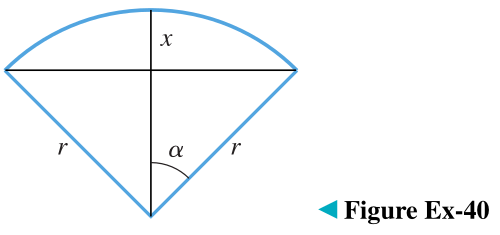
\includegraphics[width=0.5\textwidth]{../img/img_Lista2/2_40.png}
\end{figure}
\begin{enumerate}[label=(\alph*)]
\item La figura adjunta muestra un sector de radio $r$ y ángulo central $2 \alpha$. Suponiendo que el ángulo $\alpha$ es pequeño, utilice la aproximación cuadrática local de $\cos \alpha$ en $\alpha = 0$ para demostrar que $x \approx r \alpha ^2/2$. \\
La aproximación cuadrática local de $\cos \alpha$ en $\alpha = 0$ se obtiene con el polinomio de Maclaurin
\[
p_2(\alpha) = \sum_{k=0}^{2}\frac{f^{(k)} (0)}{k!} \alpha^k =  f(0) + f'(0)\alpha+ \frac{f''(0)}{2!}\alpha^2 
\] 
\begin{flushright}
(1)
\end{flushright}
\begin{center}
  \begin{tabular}{r l}
   $f(\alpha) = cos\alpha $ & $ f(0) = cos(0) = 1$ \\
   $f'(\alpha) = \frac{d}{d\alpha} cosx = -sen\alpha$ & $ f'(0) = -sen(0) = 0$ \\
   $f''(\alpha) = \frac{d^2}{d\alpha^2} cos \alpha = \frac{d}{d\alpha} -sen \alpha = -cosx$ & $ f''(0) = -cos(0) = -1$ \\
  \end{tabular}
\end{center}
Sustituyendo en (1)
\[
cos\alpha \approx 1 + 0 \alpha+ \frac{-1}{2}\alpha^2 = 1 - \frac{\alpha^2}{2} 
\]
\begin{flushright}
(2)
\end{flushright}


Observando la figura podemos concluir que $x = r - z$ (3) donde z es el cateto adyacente al triángulo rectangulo donde encontramos $\alpha$.
Bajo estos términos, $cos\alpha = \frac{z}{r} $ así que $z = cos \alpha \cdot r$.\\
Sustituyendo z  en (3) obtenemos $x = r -(cos \alpha \cdot r) $ (4).\\
Remplazando $cos\alpha$  en (4) por su aproximación antes obtenida en (2), obtenemos que 
\begin{eqnarray}
x
& = &  r -(cos \alpha \cdot r) \nonumber
\\
& \approx & r -(r \cdot (1 - \frac{\alpha^2}{2})) \nonumber
\\
& \approx  & r -(r - \frac{\alpha^2 \cdot r}{2}) \nonumber
\\
& \approx & r -r + \frac{\alpha^2 \cdot r}{2}) \nonumber
\\
& \approx & \frac{\alpha^2 \cdot r}{2} \nonumber
\end{eqnarray}
\[
\therefore x \approx \frac{r \cdot \alpha^2 }{2}
\]
\item Suponiendo que la Tierra es una esfera de radio $4000 mi$, use el resultado del inciso $(a)$ para aproximar la cantidad máxima en la que un arco de $100 mi$ a lo largo del ecuador divergirá de su cuerda.\\
Encontrar cantidad en la que un arco de la Tierra divergira del ecuador es equivalente a encontra $x$ en el inciso anterior.
Para usar $x \approx \frac{r \cdot \alpha^2 }{2}$ conocemos que el radio es de 4000 mi pero necesitamos conocer el ángulo támbien. \\
Conocemos que el tamaño del arco es de 100 mi y este se puede calcular dar en términos del radio y el ángulo, siendo que:
\[
c = r \cdot \theta
\]
donde:
c es el tamaño del arco,
r es el radio,
$\theta$ es el ángulo que genera el segmento.
Despejando, podemos calcular el ángulo $\theta$:
\[
\theta = \frac{c}{r}
\]
Remplazando por los datos conocidos:
\[
\theta = \frac{100}{4000} = 0.025 rad
\]
Sin embargo, la ecuación segun la figura esta dada para un ángulo $\alpha$ que es la mitad del ángulo $\theta$ que corresponde al del total del segmento.	Así que
\[
\alpha = \frac{\theta}{2} = \frac{0.025}{2}= 0.0125 rad
\]
Una vez conocidos todos los valores necesarios, podemos aplicar la fórmula para x
\begin{eqnarray}
x
& \approx &  \frac{r \cdot \alpha^2 }{2} \nonumber
\\
& \approx & \frac{4000 \cdot 0.0125^2 }{2} \nonumber
\\
& \approx  & 0.3125 ~ mi\nonumber
\\
\end{eqnarray}
$\therefore$  La cantidad máxima en la que un arco de $100 mi$ a lo largo del ecuador divergirá de su cuerda es 0.3125 mi.

\end{enumerate}


%% 6
\section{Identidad de Euler} name \\

Aplicar las definiciones de las funciones exponencial natural, seno y coseno como series de Taylor para demostrar la identidad de Euler:
\[e^{i\theta} = \cos(\theta) + i \sin(\theta)\]
y deducir, de aquí, que:
\[exp(i\pi) + 1 = 0\]

Para demostrar que $e^{i\theta} = \cos(\theta) + i \sin(\theta)$ hay que considerar las sigueintes definiciones:
\[
e^x = \sum_{k=0}^{\infty}\frac{x^{k}}{k!}
\]

\[
\cos\theta = \sum_{k=0}^{\infty}\frac{(-1)^{k}}{2k!} \cdot \theta ^{2k} = 1- \frac{\theta^2}{2!} + \frac{\theta ^4}{4!} -   \frac{\theta^6}{6!} + \ldots
\]
\[
\sin\theta = \sum_{k=0}^{\infty}\frac{(-1)^{k}}{(2k+1)!} \cdot \theta ^{2k+1} =  \theta - \frac{\theta^3}{3!} + \frac{\theta ^5}{5!} -   \frac{\theta^7}{7!} + \ldots
\]
Podemos desarrollar la función de exponencial natural como serie de Taylor
\[
e^{i\theta} = \sum_{k=0}^{\infty}\frac{(i\theta)^{k}}{k!} = 1 + i\theta+ \frac{(i\theta)^2}{2!} + \frac{(i\theta)^3}{3!}+ \frac{(i\theta)^4}{4!}+ \frac{(i\theta)^5}{5!} + \frac{(i\theta)^6}{6!} + \frac{(i\theta)^7}{7!}     
\]
\begin{eqnarray}
e^{i\theta} 
& = &   \sum_{k=0}^{\infty}\frac{(i\theta)^{k}}{k!} \nonumber
\\
& = & 1 + i\theta + \frac{(i\theta)^2}{2!} + \frac{(i\theta)^3}{3!}+ \frac{(i\theta)^4}{4!}+ \frac{(i\theta)^5}{5!} + \frac{(i\theta)^6}{6!} + \frac{(i\theta)^7}{7!}+ \ldots  \nonumber
\\
& = &  1 + i\theta - \frac{\theta^2}{2!} - \frac{(i\theta)^3}{3!}+ \frac{\theta^4}{4!}+ \frac{(i\theta)^5}{5!} - \frac{\theta^6}{6!} - \frac{(i\theta)^7}{7!}+ \ldots  \nonumber
\\\nonumber
\end{eqnarray}
Al agrupar los terminos complejos y los reales.
\begin{eqnarray}
e^{i\theta} 
& = &  1 + i\theta - \frac{\theta^2}{2!} - \frac{(i\theta)^3}{3!}+ \frac{\theta^4}{4!}+ \frac{(i\theta)^5}{5!} - \frac{\theta^6}{6!} - \frac{(i\theta)^7}{7!}+ \ldots  \nonumber
\\
& = &  [1 - \frac{\theta^2}{2!} + \frac{\theta^4}{4!}- \frac{\theta^6}{6!} + \ldots ]+[i\theta   - \frac{(i\theta)^3}{3!}+ \frac{(i\theta)^5}{5!} - \frac{(i\theta)^7}{7!}+ \ldots]  \nonumber
\\
& = &  [1 - \frac{\theta^2}{2!} + \frac{\theta^4}{4!}- \frac{\theta^6}{6!} + \ldots ]+i[\theta   - \frac{(\theta)^3}{3!}+ \frac{(\theta)^5}{5!} - \frac{(\theta)^7}{7!}+ \ldots]  \nonumber
\\\nonumber
\end{eqnarray}
Estos grupos son las definiciones de $\cos\theta$ y $\sin\theta$
\begin{eqnarray}
e^{i\theta} \nonumber
& = &  [1 - \frac{\theta^2}{2!} + \frac{\theta^4}{4!}- \frac{\theta^6}{6!} + \ldots ]+i[\theta   - \frac{(\theta)^3}{3!}+ \frac{(\theta)^5}{5!} - \frac{(\theta)^7}{7!}+ \ldots]  \nonumber
\\
& = & \sum_{k=0}^{\infty}\frac{(-1)^{k}}{2k!} \cdot \theta ^{2k} +i [\sum_{k=0}^{\infty}\frac{(-1)^{k}}{(2k+1)!} \cdot \theta ^{2k+1}] \nonumber
\\
& = & \cos\theta +i [\sin\theta] \nonumber
\\ \nonumber
\end{eqnarray}
\[
\therefore e^{i\theta} = \cos(\theta) + i \sin(\theta)
\]
Con este resultado, sustituyendo $\theta$ por $\pi$ :
\begin{eqnarray}
e^{i\pi} \nonumber
& = &  \cos(\pi) + i \sin(\pi) \nonumber
\\
& = &  -1 + i (0) \nonumber
\\
& = &  -1\nonumber
\\ \nonumber
\end{eqnarray}
Considerando $e^{i\pi} = -1$, se puede deducir que 
\[
e^{i\pi} +1 = 0
\]
\end{document}
